% Options for packages loaded elsewhere
\PassOptionsToPackage{unicode}{hyperref}
\PassOptionsToPackage{hyphens}{url}
\PassOptionsToPackage{dvipsnames,svgnames,x11names}{xcolor}
%
\documentclass[
  letterpaper,
  DIV=11,
  numbers=noendperiod]{scrreprt}

\usepackage{amsmath,amssymb}
\usepackage{lmodern}
\usepackage{iftex}
\ifPDFTeX
  \usepackage[T1]{fontenc}
  \usepackage[utf8]{inputenc}
  \usepackage{textcomp} % provide euro and other symbols
\else % if luatex or xetex
  \usepackage{unicode-math}
  \defaultfontfeatures{Scale=MatchLowercase}
  \defaultfontfeatures[\rmfamily]{Ligatures=TeX,Scale=1}
\fi
% Use upquote if available, for straight quotes in verbatim environments
\IfFileExists{upquote.sty}{\usepackage{upquote}}{}
\IfFileExists{microtype.sty}{% use microtype if available
  \usepackage[]{microtype}
  \UseMicrotypeSet[protrusion]{basicmath} % disable protrusion for tt fonts
}{}
\makeatletter
\@ifundefined{KOMAClassName}{% if non-KOMA class
  \IfFileExists{parskip.sty}{%
    \usepackage{parskip}
  }{% else
    \setlength{\parindent}{0pt}
    \setlength{\parskip}{6pt plus 2pt minus 1pt}}
}{% if KOMA class
  \KOMAoptions{parskip=half}}
\makeatother
\usepackage{xcolor}
\setlength{\emergencystretch}{3em} % prevent overfull lines
\setcounter{secnumdepth}{5}
% Make \paragraph and \subparagraph free-standing
\ifx\paragraph\undefined\else
  \let\oldparagraph\paragraph
  \renewcommand{\paragraph}[1]{\oldparagraph{#1}\mbox{}}
\fi
\ifx\subparagraph\undefined\else
  \let\oldsubparagraph\subparagraph
  \renewcommand{\subparagraph}[1]{\oldsubparagraph{#1}\mbox{}}
\fi

\usepackage{color}
\usepackage{fancyvrb}
\newcommand{\VerbBar}{|}
\newcommand{\VERB}{\Verb[commandchars=\\\{\}]}
\DefineVerbatimEnvironment{Highlighting}{Verbatim}{commandchars=\\\{\}}
% Add ',fontsize=\small' for more characters per line
\usepackage{framed}
\definecolor{shadecolor}{RGB}{241,243,245}
\newenvironment{Shaded}{\begin{snugshade}}{\end{snugshade}}
\newcommand{\AlertTok}[1]{\textcolor[rgb]{0.68,0.00,0.00}{#1}}
\newcommand{\AnnotationTok}[1]{\textcolor[rgb]{0.37,0.37,0.37}{#1}}
\newcommand{\AttributeTok}[1]{\textcolor[rgb]{0.40,0.45,0.13}{#1}}
\newcommand{\BaseNTok}[1]{\textcolor[rgb]{0.68,0.00,0.00}{#1}}
\newcommand{\BuiltInTok}[1]{\textcolor[rgb]{0.00,0.23,0.31}{#1}}
\newcommand{\CharTok}[1]{\textcolor[rgb]{0.13,0.47,0.30}{#1}}
\newcommand{\CommentTok}[1]{\textcolor[rgb]{0.37,0.37,0.37}{#1}}
\newcommand{\CommentVarTok}[1]{\textcolor[rgb]{0.37,0.37,0.37}{\textit{#1}}}
\newcommand{\ConstantTok}[1]{\textcolor[rgb]{0.56,0.35,0.01}{#1}}
\newcommand{\ControlFlowTok}[1]{\textcolor[rgb]{0.00,0.23,0.31}{#1}}
\newcommand{\DataTypeTok}[1]{\textcolor[rgb]{0.68,0.00,0.00}{#1}}
\newcommand{\DecValTok}[1]{\textcolor[rgb]{0.68,0.00,0.00}{#1}}
\newcommand{\DocumentationTok}[1]{\textcolor[rgb]{0.37,0.37,0.37}{\textit{#1}}}
\newcommand{\ErrorTok}[1]{\textcolor[rgb]{0.68,0.00,0.00}{#1}}
\newcommand{\ExtensionTok}[1]{\textcolor[rgb]{0.00,0.23,0.31}{#1}}
\newcommand{\FloatTok}[1]{\textcolor[rgb]{0.68,0.00,0.00}{#1}}
\newcommand{\FunctionTok}[1]{\textcolor[rgb]{0.28,0.35,0.67}{#1}}
\newcommand{\ImportTok}[1]{\textcolor[rgb]{0.00,0.46,0.62}{#1}}
\newcommand{\InformationTok}[1]{\textcolor[rgb]{0.37,0.37,0.37}{#1}}
\newcommand{\KeywordTok}[1]{\textcolor[rgb]{0.00,0.23,0.31}{#1}}
\newcommand{\NormalTok}[1]{\textcolor[rgb]{0.00,0.23,0.31}{#1}}
\newcommand{\OperatorTok}[1]{\textcolor[rgb]{0.37,0.37,0.37}{#1}}
\newcommand{\OtherTok}[1]{\textcolor[rgb]{0.00,0.23,0.31}{#1}}
\newcommand{\PreprocessorTok}[1]{\textcolor[rgb]{0.68,0.00,0.00}{#1}}
\newcommand{\RegionMarkerTok}[1]{\textcolor[rgb]{0.00,0.23,0.31}{#1}}
\newcommand{\SpecialCharTok}[1]{\textcolor[rgb]{0.37,0.37,0.37}{#1}}
\newcommand{\SpecialStringTok}[1]{\textcolor[rgb]{0.13,0.47,0.30}{#1}}
\newcommand{\StringTok}[1]{\textcolor[rgb]{0.13,0.47,0.30}{#1}}
\newcommand{\VariableTok}[1]{\textcolor[rgb]{0.07,0.07,0.07}{#1}}
\newcommand{\VerbatimStringTok}[1]{\textcolor[rgb]{0.13,0.47,0.30}{#1}}
\newcommand{\WarningTok}[1]{\textcolor[rgb]{0.37,0.37,0.37}{\textit{#1}}}

\providecommand{\tightlist}{%
  \setlength{\itemsep}{0pt}\setlength{\parskip}{0pt}}\usepackage{longtable,booktabs,array}
\usepackage{calc} % for calculating minipage widths
% Correct order of tables after \paragraph or \subparagraph
\usepackage{etoolbox}
\makeatletter
\patchcmd\longtable{\par}{\if@noskipsec\mbox{}\fi\par}{}{}
\makeatother
% Allow footnotes in longtable head/foot
\IfFileExists{footnotehyper.sty}{\usepackage{footnotehyper}}{\usepackage{footnote}}
\makesavenoteenv{longtable}
\usepackage{graphicx}
\makeatletter
\def\maxwidth{\ifdim\Gin@nat@width>\linewidth\linewidth\else\Gin@nat@width\fi}
\def\maxheight{\ifdim\Gin@nat@height>\textheight\textheight\else\Gin@nat@height\fi}
\makeatother
% Scale images if necessary, so that they will not overflow the page
% margins by default, and it is still possible to overwrite the defaults
% using explicit options in \includegraphics[width, height, ...]{}
\setkeys{Gin}{width=\maxwidth,height=\maxheight,keepaspectratio}
% Set default figure placement to htbp
\makeatletter
\def\fps@figure{htbp}
\makeatother

\KOMAoption{captions}{tableheading}
\makeatletter
\makeatother
\makeatletter
\@ifpackageloaded{bookmark}{}{\usepackage{bookmark}}
\makeatother
\makeatletter
\@ifpackageloaded{caption}{}{\usepackage{caption}}
\AtBeginDocument{%
\ifdefined\contentsname
  \renewcommand*\contentsname{Table of contents}
\else
  \newcommand\contentsname{Table of contents}
\fi
\ifdefined\listfigurename
  \renewcommand*\listfigurename{List of Figures}
\else
  \newcommand\listfigurename{List of Figures}
\fi
\ifdefined\listtablename
  \renewcommand*\listtablename{List of Tables}
\else
  \newcommand\listtablename{List of Tables}
\fi
\ifdefined\figurename
  \renewcommand*\figurename{Figure}
\else
  \newcommand\figurename{Figure}
\fi
\ifdefined\tablename
  \renewcommand*\tablename{Table}
\else
  \newcommand\tablename{Table}
\fi
}
\@ifpackageloaded{float}{}{\usepackage{float}}
\floatstyle{ruled}
\@ifundefined{c@chapter}{\newfloat{codelisting}{h}{lop}}{\newfloat{codelisting}{h}{lop}[chapter]}
\floatname{codelisting}{Listing}
\newcommand*\listoflistings{\listof{codelisting}{List of Listings}}
\makeatother
\makeatletter
\@ifpackageloaded{caption}{}{\usepackage{caption}}
\@ifpackageloaded{subcaption}{}{\usepackage{subcaption}}
\makeatother
\makeatletter
\@ifpackageloaded{tcolorbox}{}{\usepackage[many]{tcolorbox}}
\makeatother
\makeatletter
\@ifundefined{shadecolor}{\definecolor{shadecolor}{rgb}{.97, .97, .97}}
\makeatother
\makeatletter
\makeatother
\ifLuaTeX
  \usepackage{selnolig}  % disable illegal ligatures
\fi
\IfFileExists{bookmark.sty}{\usepackage{bookmark}}{\usepackage{hyperref}}
\IfFileExists{xurl.sty}{\usepackage{xurl}}{} % add URL line breaks if available
\urlstyle{same} % disable monospaced font for URLs
\hypersetup{
  pdftitle={Emre Çakmak Progress Journal},
  colorlinks=true,
  linkcolor={blue},
  filecolor={Maroon},
  citecolor={Blue},
  urlcolor={Blue},
  pdfcreator={LaTeX via pandoc}}

\title{Emre Çakmak Progress Journal}
\author{}
\date{}

\begin{document}
\maketitle
\ifdefined\Shaded\renewenvironment{Shaded}{\begin{tcolorbox}[enhanced, boxrule=0pt, sharp corners, borderline west={3pt}{0pt}{shadecolor}, breakable, interior hidden, frame hidden]}{\end{tcolorbox}}\fi

\renewcommand*\contentsname{Table of contents}
{
\hypersetup{linkcolor=}
\setcounter{tocdepth}{2}
\tableofcontents
}
\bookmarksetup{startatroot}

\hypertarget{introduction}{%
\chapter*{Introduction}\label{introduction}}
\addcontentsline{toc}{chapter}{Introduction}

This progress journal covers Emre Çakmak's work during their term at
\href{https://mef-bda503.github.io/fall22/}{BDA 503 Fall 2022}.

Each section is an assignment or an individual work.

\bookmarksetup{startatroot}

\hypertarget{bda-503-assigment-1}{%
\chapter{BDA-503 Assigment 1}\label{bda-503-assigment-1}}

A short brief of author and R use cases

Emre Çakmak\\
2022-10-09

\hfill\break

Hi dear reader,

I'm Emre Çakmak from Istanbul/Turkey. I graduated from my bachelor at
Istanbul Technical University, Industrial Engineering Department in
2018.

My current role is Data Scientist at E-commerce Department in LC Waikiki
which is a Istanbul based global fashion retailer driving operations on
more than 50 countries. I had different positions like Data Analyst,
Business Intelligence Specialist in different companies during past 4
years. Especially in last 1 year, I dedicated to improve myself for
application of ML Technics due to enrich customer\&item based data. So,
I'm a part of BDA Graduate Program in MEF University to wide my
knowledge in audience management and marketing applications by the help
of real-life use cases.

\href{https://www.linkedin.com/in/emre-\%C3\%A7akmak-7778b160/}{\textbf{Here
is my LinkedIn Profile}}

\begin{figure}

\href{https://www.linkedin.com/in/emre-\%C3\%A7akmak-7778b160/}{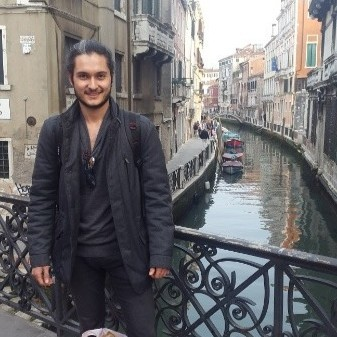
\includegraphics[width=1.04167in,height=\textheight]{./images/emrecakmak.png}}

\end{figure}

\hypertarget{rstudio-global-2022-conference---quarto-for-the-curious}{%
\section{RStudio Global 2022 Conference - Quarto for the
Curious}\label{rstudio-global-2022-conference---quarto-for-the-curious}}

\href{https://www.rstudio.com/conference/2022/talks/quarto-for-rmarkdown-users/}{What's
\emph{Quarto} according to Tom Mock}

In this paragraph, I aim to give you some main differences between
\emph{Quarto,} the brand new documentation system which has been
released April 2022, and \emph{RMarkdown} being used for almost a
decade.

\begin{itemize}
\tightlist
\item
  Tom Mock says \emph{Quarto} is Open source scientific and technical
  publishing system. Also he added that \emph{Quarto} is the next
  generation of \emph{RMarkdown}.
\end{itemize}

Here is some differences between them:

\hypertarget{preprocessing}{%
\subsection{Preprocessing}\label{preprocessing}}

\begin{figure}

\begin{minipage}[t]{0.50\linewidth}

{\centering 

\raisebox{-\height}{

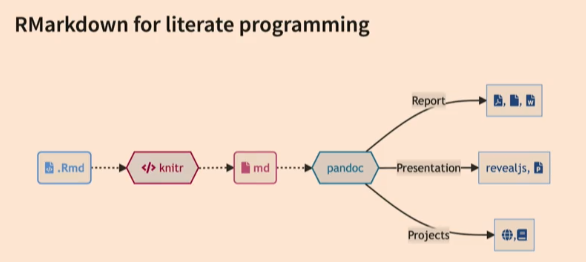
\includegraphics[width=3.64583in,height=\textheight]{./images/rmarkdown.PNG}

}

}

\subcaption{\label{fig-rmarkdown}RMarkdown}
\end{minipage}%
%
\begin{minipage}[t]{0.50\linewidth}

{\centering 

\raisebox{-\height}{

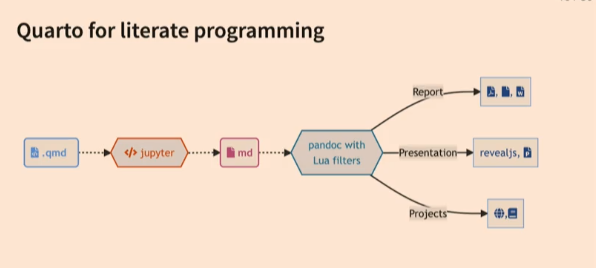
\includegraphics[width=3.64583in,height=\textheight]{./images/quatro.PNG}

}

}

\subcaption{\label{fig-quatro}Quarto}
\end{minipage}%

\caption{\label{fig-quarto-vs-rmarkdown}RMarkdown vs Quarto
Preprocessing Diagram}

\end{figure}

Altough it seems like they have almost same workflow behind the scenes;
\emph{Quarto} doesn't need to have R in the system to use it. It means
that you can use \emph{Quarto} in a fresh computer but \emph{Rmarkdown}
needs to have R in the system.

\hypertarget{language-support}{%
\subsection{Language Support}\label{language-support}}

The main purpose of releasing \emph{Quarto} is improving the
communication between data science communities whatever their language
is. Because of this \emph{Quarto} supports other languages as engine.

\begin{figure}

{\centering 

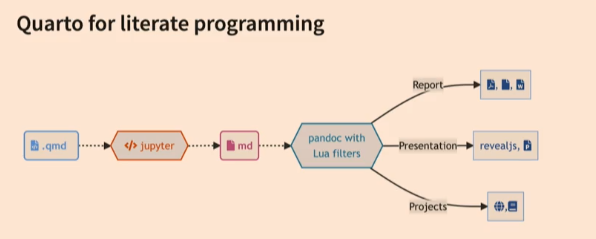
\includegraphics[width=3.64583in,height=\textheight]{./images/quartojupytersupport.PNG}

}

\caption{\label{fig-quarto-language-support}Jupyter as Quarto Engine}

\end{figure}

This availability in \emph{Quarto} and not limiting with R allows people
to collaborate as Python developer with others. Tom Mock figured this
situation out like

\begin{itemize}
\tightlist
\item
  \textbf{Quarto: Comfortable baking in your own kitchen}
\item
  \textbf{RMarkdown: Uncomfortable baking in corporate kitchen}
\end{itemize}

\hypertarget{r-posts}{%
\section{R Posts}\label{r-posts}}

This section includes 3 different R Programming use case

\hypertarget{web-scraping-with-r}{%
\subsection{Web Scraping with R}\label{web-scraping-with-r}}

It's very known fact that people have some struggle to access to a clean
dataset. In these cases, we need to be a little bit creative to create
our own dataset. And one way of the creating a new dataset is web
scraping.

In this paragraph, I want to introduce how to scrape a web page by the
help of R packages. The most common 2 packages are:

\begin{itemize}
\tightlist
\item
  \{rvest\}
\item
  \{RSelenium\}
\end{itemize}

\textbf{Note that: Some websites have strict policies against scraping.
Be careful!}

Step by step scraping of public IMDB Dataset

\textbf{Step 1: Install Package}

\begin{Shaded}
\begin{Highlighting}[]
\DocumentationTok{\#\# Before you start, you need to execute once the code below.}
\DocumentationTok{\#\#install.packages("rvest")}
\end{Highlighting}
\end{Shaded}

\textbf{Step 2: Call the library and use html functions}

\begin{Shaded}
\begin{Highlighting}[]
\DocumentationTok{\#\# call the rvest library for required functions}
\FunctionTok{library}\NormalTok{(rvest)}

\DocumentationTok{\#\# define the website link you want to scrape}
\NormalTok{link }\OtherTok{=} \StringTok{"https://www.imdb.com/search/title/?title\_type=feature\&num\_votes=30000,\&genres=comedy"}

\DocumentationTok{\#\# send a http get request to the link above and store it in a variable}
\NormalTok{page }\OtherTok{=} \FunctionTok{read\_html}\NormalTok{(link)}

\DocumentationTok{\#\# filter and grab all elements in same class}
\NormalTok{titles }\OtherTok{=}\NormalTok{ page }\SpecialCharTok{\%\textgreater{}\%} \FunctionTok{html\_nodes}\NormalTok{(}\StringTok{".lister{-}item{-}header a"}\NormalTok{) }\SpecialCharTok{\%\textgreater{}\%} \FunctionTok{html\_text}\NormalTok{()}

\DocumentationTok{\#\# preview the titles}
\NormalTok{titles[}\DecValTok{1}\SpecialCharTok{:}\DecValTok{10}\NormalTok{]}
\end{Highlighting}
\end{Shaded}

\begin{verbatim}
 [1] "Bullet Train"                         
 [2] "A Christmas Story"                    
 [3] "Enchanted"                            
 [4] "Everything Everywhere All at Once"    
 [5] "Thor: Love and Thunder"               
 [6] "The Bad Guys"                         
 [7] "Home Alone"                           
 [8] "Knives Out"                           
 [9] "National Lampoon's Christmas Vacation"
[10] "The Santa Clause"                     
\end{verbatim}

\textbf{Step 3: Create other variables}

\begin{Shaded}
\begin{Highlighting}[]
\DocumentationTok{\#\# apply same procedure to other variables}
\NormalTok{year}\OtherTok{=}\NormalTok{ page }\SpecialCharTok{\%\textgreater{}\%} \FunctionTok{html\_nodes}\NormalTok{(}\StringTok{".text{-}muted.unbold"}\NormalTok{) }\SpecialCharTok{\%\textgreater{}\%} \FunctionTok{html\_text}\NormalTok{()}
\NormalTok{rating }\OtherTok{=}\NormalTok{ page }\SpecialCharTok{\%\textgreater{}\%} \FunctionTok{html\_nodes}\NormalTok{(}\StringTok{".ratings{-}imdb{-}rating strong"}\NormalTok{) }\SpecialCharTok{\%\textgreater{}\%} \FunctionTok{html\_text}\NormalTok{()}


\DocumentationTok{\#\# preview variables}
\NormalTok{year[}\DecValTok{1}\SpecialCharTok{:}\DecValTok{10}\NormalTok{]}
\end{Highlighting}
\end{Shaded}

\begin{verbatim}
 [1] "(2022)" "(1983)" "(2007)" "(2022)" "(2022)" "(2022)" "(1990)" "(2019)"
 [9] "(1989)" "(1994)"
\end{verbatim}

\begin{Shaded}
\begin{Highlighting}[]
\NormalTok{rating[}\DecValTok{1}\SpecialCharTok{:}\DecValTok{10}\NormalTok{]}
\end{Highlighting}
\end{Shaded}

\begin{verbatim}
 [1] "7.3" "7.9" "7.1" "8.1" "6.3" "6.8" "7.7" "7.9" "7.5" "6.5"
\end{verbatim}

\textbf{Step 4: Create data frame}

\begin{Shaded}
\begin{Highlighting}[]
\DocumentationTok{\#\# create a dataset}
\NormalTok{movies }\OtherTok{=} \FunctionTok{data.frame}\NormalTok{(titles, year, rating, }\AttributeTok{stringsAsFactors =} \ConstantTok{FALSE}\NormalTok{)}
\NormalTok{movies[}\DecValTok{1}\SpecialCharTok{:}\DecValTok{10}\NormalTok{,]}
\end{Highlighting}
\end{Shaded}

\begin{verbatim}
                                  titles   year rating
1                           Bullet Train (2022)    7.3
2                      A Christmas Story (1983)    7.9
3                              Enchanted (2007)    7.1
4      Everything Everywhere All at Once (2022)    8.1
5                 Thor: Love and Thunder (2022)    6.3
6                           The Bad Guys (2022)    6.8
7                             Home Alone (1990)    7.7
8                             Knives Out (2019)    7.9
9  National Lampoon's Christmas Vacation (1989)    7.5
10                      The Santa Clause (1994)    6.5
\end{verbatim}

References of web scraping with R:

\begin{itemize}
\tightlist
\item
  \href{https://www.scraperapi.com/blog/web-scraping-with-r/}{Scraperapi}
\item
  \href{https://www.scrapingbee.com/blog/web-scraping-r/}{Scrapingbee}
\item
  \href{https://appsilon.com/webscraping-dynamic-websites-with-r/}{Appsilon}
\end{itemize}

\hypertarget{simple-aggregations-on-dataset}{%
\subsection{Simple Aggregations on
Dataset}\label{simple-aggregations-on-dataset}}

This part provides some basic aggregations and data manipulation methods
in R via \{dplyr\} package.

Without leaving the concept in previous part, we can assume that we
created our own dataset. So, what's next?

The process of extracting insightful information from datasets starts
from understanding the data structure and manipulating them. R provides
a package just for this: \textbf{\{dplyr\}}

Step by step aggregation \& filtering \& summarizing dataset

\textbf{Step 1: Install Package}

\begin{Shaded}
\begin{Highlighting}[]
\DocumentationTok{\#\# Before you start, you need to execute once the code below.}
\DocumentationTok{\#\#install.packages("dplyr")}
\end{Highlighting}
\end{Shaded}

\textbf{Step 2: Call the library}

\begin{Shaded}
\begin{Highlighting}[]
\FunctionTok{library}\NormalTok{(dplyr)}
\end{Highlighting}
\end{Shaded}

\begin{verbatim}

Attaching package: 'dplyr'
\end{verbatim}

\begin{verbatim}
The following objects are masked from 'package:stats':

    filter, lag
\end{verbatim}

\begin{verbatim}
The following objects are masked from 'package:base':

    intersect, setdiff, setequal, union
\end{verbatim}

\textbf{Step 3: Select subset of data in different aspects}

\begin{Shaded}
\begin{Highlighting}[]
\DocumentationTok{\#\# selecting specific columns}
\FunctionTok{select}\NormalTok{(movies, titles, year)[}\DecValTok{1}\SpecialCharTok{:}\DecValTok{10}\NormalTok{,]}
\end{Highlighting}
\end{Shaded}

\begin{verbatim}
                                  titles   year
1                           Bullet Train (2022)
2                      A Christmas Story (1983)
3                              Enchanted (2007)
4      Everything Everywhere All at Once (2022)
5                 Thor: Love and Thunder (2022)
6                           The Bad Guys (2022)
7                             Home Alone (1990)
8                             Knives Out (2019)
9  National Lampoon's Christmas Vacation (1989)
10                      The Santa Clause (1994)
\end{verbatim}

\begin{Shaded}
\begin{Highlighting}[]
\DocumentationTok{\#\# filter data according to specific condition}
\FunctionTok{filter}\NormalTok{(movies, rating }\SpecialCharTok{\textgreater{}} \DecValTok{8}\NormalTok{)}
\end{Highlighting}
\end{Shaded}

\begin{verbatim}
                             titles   year rating
1 Everything Everywhere All at Once (2022)    8.1
2           The Wolf of Wall Street (2013)    8.2
3                Back to the Future (1985)    8.5
4                          Zootopia (2016)    8.0
5                          Deadpool (2016)    8.0
6           Guardians of the Galaxy (2014)    8.0
7                   The Truman Show (1998)    8.2
\end{verbatim}

\begin{Shaded}
\begin{Highlighting}[]
\DocumentationTok{\#\# sort rows}
\FunctionTok{arrange}\NormalTok{(movies, }\FunctionTok{desc}\NormalTok{(titles))[}\DecValTok{1}\SpecialCharTok{:}\DecValTok{10}\NormalTok{,]}
\end{Highlighting}
\end{Shaded}

\begin{verbatim}
                                    titles   year rating
1                                 Zootopia (2016)    8.0
2                   Thor: Love and Thunder (2022)    6.3
3                  The Wolf of Wall Street (2013)    8.2
4  The Unbearable Weight of Massive Talent (2022)    7.0
5                          The Truman Show (1998)    8.2
6                             The Terminal (2004)    7.4
7                        The Suicide Squad (2021)    7.2
8                       The Santa Clause 2 (2002)    5.7
9                         The Santa Clause (1994)    6.5
10                       The Polar Express (2004)    6.6
\end{verbatim}

\begin{Shaded}
\begin{Highlighting}[]
\DocumentationTok{\#\# select top n rows}
\FunctionTok{top\_n}\NormalTok{(movies, }\DecValTok{3}\NormalTok{, titles)}
\end{Highlighting}
\end{Shaded}

\begin{verbatim}
                   titles   year rating
1  Thor: Love and Thunder (2022)    6.3
2 The Wolf of Wall Street (2013)    8.2
3                Zootopia (2016)    8.0
\end{verbatim}

\textbf{Step 4: Summarize Dataset}

\begin{Shaded}
\begin{Highlighting}[]
\DocumentationTok{\#\# convert rating columns as numeric and calculate the average}
\FunctionTok{summarise}\NormalTok{(movies, }\AttributeTok{average\_rating =} \FunctionTok{mean}\NormalTok{(}\FunctionTok{as.numeric}\NormalTok{(rating)))}
\end{Highlighting}
\end{Shaded}

\begin{verbatim}
  average_rating
1          7.176
\end{verbatim}

\begin{Shaded}
\begin{Highlighting}[]
\DocumentationTok{\#\# group by and summarize}
\NormalTok{grouped\_data }\OtherTok{=} \FunctionTok{group\_by}\NormalTok{(movies, year)}
\FunctionTok{summarise}\NormalTok{(grouped\_data, }\AttributeTok{average\_rating =} \FunctionTok{mean}\NormalTok{(}\FunctionTok{as.numeric}\NormalTok{(rating)))[}\DecValTok{1}\SpecialCharTok{:}\DecValTok{5}\NormalTok{,]}
\end{Highlighting}
\end{Shaded}

\begin{verbatim}
# A tibble: 5 x 2
  year   average_rating
  <chr>           <dbl>
1 (1983)            7.9
2 (1984)            7.8
3 (1985)            8.1
4 (1987)            7.6
5 (1989)            7.5
\end{verbatim}

\textbf{Step 5: \%\textgreater\% Operator}

This operator takes the object from the left and gives it as the first
argument to the function on the right. It makes your code more readable.

\begin{Shaded}
\begin{Highlighting}[]
\DocumentationTok{\#\# same grouping and summarizing operation at step4 }

\NormalTok{movies }\SpecialCharTok{\%\textgreater{}\%}
  \FunctionTok{group\_by}\NormalTok{(year) }\SpecialCharTok{\%\textgreater{}\%}
  \FunctionTok{summarise}\NormalTok{(}\AttributeTok{average\_rating =} \FunctionTok{mean}\NormalTok{(}\FunctionTok{as.numeric}\NormalTok{(rating)))}\SpecialCharTok{\%\textgreater{}\%}
  \FunctionTok{top\_n}\NormalTok{(}\DecValTok{5}\NormalTok{, }\FunctionTok{desc}\NormalTok{(average\_rating))}
\end{Highlighting}
\end{Shaded}

\begin{verbatim}
# A tibble: 5 x 2
  year       average_rating
  <chr>               <dbl>
1 (1994)                6.4
2 (2000)                6.2
3 (2002)                5.7
4 (2012)                6.6
5 (I) (2022)            5.1
\end{verbatim}

Reference of aggregations with R:

\begin{itemize}
\tightlist
\item
  \href{https://courses.cs.ut.ee/MTAT.03.183/2017_fall/uploads/Main/dplyr.html}{courses.cs.ut.ee}
\end{itemize}

\hypertarget{visualization-with-r}{%
\subsection{Visualization with R}\label{visualization-with-r}}

\textbf{Step 1: Install Package}

\begin{Shaded}
\begin{Highlighting}[]
\DocumentationTok{\#\# Before you start, you need to execute once the code below.}
\DocumentationTok{\#\#install.packages("ggplot2")}
\end{Highlighting}
\end{Shaded}

\textbf{Step 2: Call the library}

\begin{Shaded}
\begin{Highlighting}[]
\FunctionTok{library}\NormalTok{(ggplot2)}
\end{Highlighting}
\end{Shaded}

\textbf{Step 3: Histogram with ggplot2}

\begin{Shaded}
\begin{Highlighting}[]
\DocumentationTok{\#\# convert rating field as numeric and keep in original dataset}
\NormalTok{movies}\SpecialCharTok{$}\NormalTok{rating}\OtherTok{=}\FunctionTok{as.numeric}\NormalTok{(rating)}

\DocumentationTok{\#\# histogram for ratings}
\FunctionTok{hist}\NormalTok{(movies}\SpecialCharTok{$}\NormalTok{rating,}\AttributeTok{col=}\StringTok{\textquotesingle{}steelblue\textquotesingle{}}\NormalTok{,}\AttributeTok{main=}\StringTok{\textquotesingle{}Rating Histogram\textquotesingle{}}\NormalTok{,}
     \AttributeTok{xlab=}\StringTok{\textquotesingle{}Ratings\textquotesingle{}}\NormalTok{)}
\end{Highlighting}
\end{Shaded}

\begin{figure}[H]

{\centering 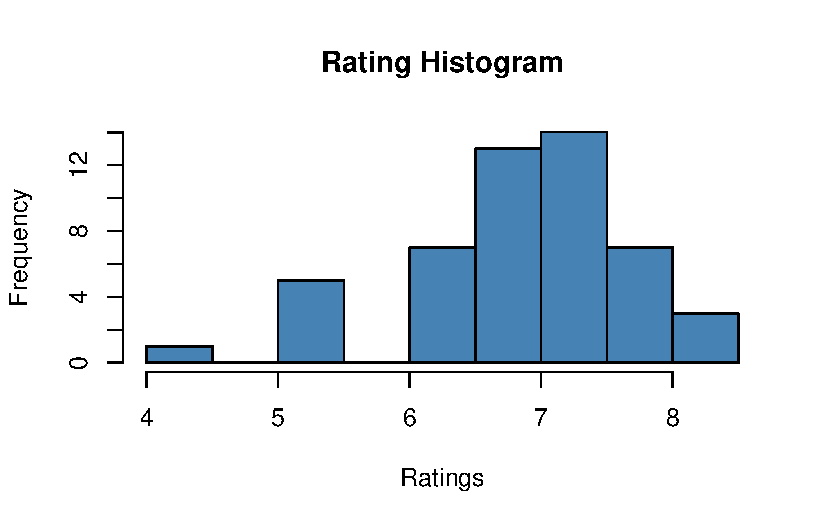
\includegraphics{./assignment1_files/figure-pdf/visualization-chunk3-1.pdf}

}

\end{figure}

\textbf{Step 4: Pie Chart with ggplot2}

\begin{Shaded}
\begin{Highlighting}[]
\DocumentationTok{\#\# Set a new flag in dataset}
\NormalTok{movies}\OtherTok{=}\NormalTok{movies }\SpecialCharTok{\%\textgreater{}\%} \FunctionTok{mutate}\NormalTok{(}\AttributeTok{rating\_flag =} \FunctionTok{case\_when}\NormalTok{(rating}\SpecialCharTok{\textgreater{}=}\DecValTok{8}\SpecialCharTok{\textasciitilde{}} \StringTok{"Higher 8"}\NormalTok{, }\ConstantTok{TRUE} \SpecialCharTok{\textasciitilde{}} \StringTok{"Lower 8"}\NormalTok{))}

\DocumentationTok{\#\# creating a new table for better visualization}
\NormalTok{count\_movies}\OtherTok{=}\NormalTok{movies }\SpecialCharTok{\%\textgreater{}\%} \FunctionTok{count}\NormalTok{(rating\_flag)}

\DocumentationTok{\#\# pie chart according to rating of movies}
\FunctionTok{ggplot}\NormalTok{(count\_movies, }\FunctionTok{aes}\NormalTok{(}\AttributeTok{x =} \StringTok{""}\NormalTok{, }\AttributeTok{y =}\NormalTok{ n, }\AttributeTok{fill =}\NormalTok{ rating\_flag)) }\SpecialCharTok{+}
  \FunctionTok{geom\_col}\NormalTok{(}\AttributeTok{color =} \StringTok{"black"}\NormalTok{) }\SpecialCharTok{+}
  \FunctionTok{geom\_label}\NormalTok{(}\FunctionTok{aes}\NormalTok{(}\AttributeTok{label =}\NormalTok{ n),}
             \AttributeTok{position =} \FunctionTok{position\_stack}\NormalTok{(}\AttributeTok{vjust =} \FloatTok{0.5}\NormalTok{),}
             \AttributeTok{show.legend =} \ConstantTok{FALSE}\NormalTok{) }\SpecialCharTok{+}
  \FunctionTok{coord\_polar}\NormalTok{(}\AttributeTok{theta =} \StringTok{"y"}\NormalTok{)}
\end{Highlighting}
\end{Shaded}

\begin{figure}[H]

{\centering 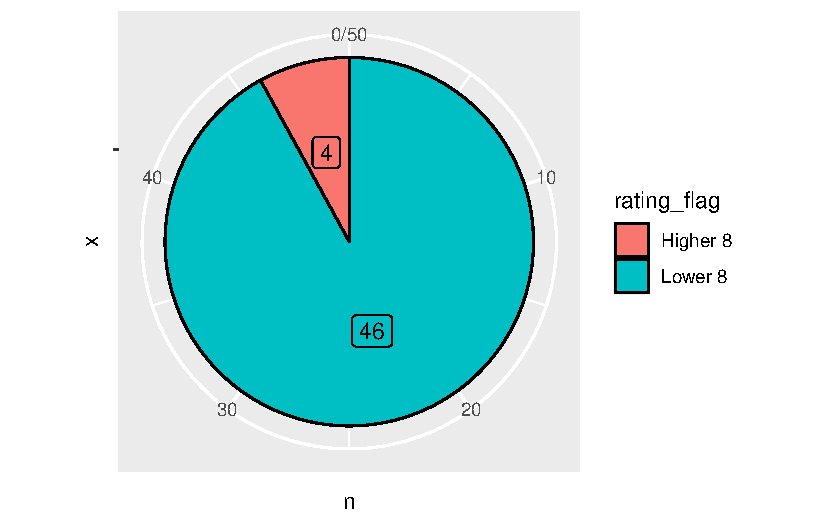
\includegraphics{./assignment1_files/figure-pdf/visualization-chunk4-1.pdf}

}

\end{figure}

References of visualization with R:

\begin{itemize}
\tightlist
\item
  \href{https://r-charts.com/part-whole/pie-chart-ggplot2/}{r-charts}
\item
  \href{https://www.kdnuggets.com/2018/06/7-simple-data-visualizations-should-know-r.html}{kdnuggets}
\end{itemize}

\bookmarksetup{startatroot}

\hypertarget{inclass-exercise-1}{%
\chapter{Inclass Exercise-1}\label{inclass-exercise-1}}

Emre Çakmak\\
2022-10-19

\hfill\break

This exercise has been prepared for understanding \{dplyr\} package
usage for functional EDA. Main data set in this exercise will be planes
data set derived from FAA.

First of all we have to install our packages.

\begin{Shaded}
\begin{Highlighting}[]
\FunctionTok{install.packages}\NormalTok{(}\StringTok{"tidyverse"}\NormalTok{)}
\FunctionTok{install.packages}\NormalTok{(}\StringTok{"nycflights13"}\NormalTok{)}
\end{Highlighting}
\end{Shaded}

Then we are calling our libraries.

\begin{Shaded}
\begin{Highlighting}[]
\FunctionTok{library}\NormalTok{(tidyverse)}
\FunctionTok{library}\NormalTok{(nycflights13)}
\end{Highlighting}
\end{Shaded}

Let's check first 10 rows of the data set. Fields and their meanings
are:

\begin{itemize}
\tightlist
\item
  \textbf{tailnum}: Tail number.
\item
  \textbf{year}: Year manufactured.
\item
  \textbf{type}: Type of plane.
\item
  \textbf{manufacturer}: Manufacturer of the aircraft.
\item
  \textbf{model}: Model of the aircraft.
\item
  \textbf{engines}: Number of engines
\item
  \textbf{seats}: Number of seats
\item
  \textbf{speed}: Average cruising speed in mph.
\item
  \textbf{engine}: Type of engine.
\end{itemize}

\begin{Shaded}
\begin{Highlighting}[]
\NormalTok{planes }\SpecialCharTok{\%\textgreater{}\%} 
  \FunctionTok{slice}\NormalTok{(}\DecValTok{1}\SpecialCharTok{:}\DecValTok{10}\NormalTok{)}
\end{Highlighting}
\end{Shaded}

\begin{verbatim}
# A tibble: 10 x 9
   tailnum  year type                   manuf~1 model engines seats speed engine
   <chr>   <int> <chr>                  <chr>   <chr>   <int> <int> <int> <chr> 
 1 N10156   2004 Fixed wing multi engi~ EMBRAER EMB-~       2    55    NA Turbo~
 2 N102UW   1998 Fixed wing multi engi~ AIRBUS~ A320~       2   182    NA Turbo~
 3 N103US   1999 Fixed wing multi engi~ AIRBUS~ A320~       2   182    NA Turbo~
 4 N104UW   1999 Fixed wing multi engi~ AIRBUS~ A320~       2   182    NA Turbo~
 5 N10575   2002 Fixed wing multi engi~ EMBRAER EMB-~       2    55    NA Turbo~
 6 N105UW   1999 Fixed wing multi engi~ AIRBUS~ A320~       2   182    NA Turbo~
 7 N107US   1999 Fixed wing multi engi~ AIRBUS~ A320~       2   182    NA Turbo~
 8 N108UW   1999 Fixed wing multi engi~ AIRBUS~ A320~       2   182    NA Turbo~
 9 N109UW   1999 Fixed wing multi engi~ AIRBUS~ A320~       2   182    NA Turbo~
10 N110UW   1999 Fixed wing multi engi~ AIRBUS~ A320~       2   182    NA Turbo~
# ... with abbreviated variable name 1: manufacturer
\end{verbatim}

\hypertarget{exercise-1}{%
\section{EXERCISE 1}\label{exercise-1}}

Now, how many aircraft does exists for each manufacturing company? Let's
calculate..

\begin{Shaded}
\begin{Highlighting}[]
\NormalTok{planes }\SpecialCharTok{\%\textgreater{}\%} 
  \FunctionTok{group\_by}\NormalTok{(manufacturer) }\SpecialCharTok{\%\textgreater{}\%} 
  \FunctionTok{summarise}\NormalTok{(}\AttributeTok{aircraft\_count =} \FunctionTok{n}\NormalTok{()) }\SpecialCharTok{\%\textgreater{}\%} 
  \FunctionTok{arrange}\NormalTok{(}\FunctionTok{desc}\NormalTok{(aircraft\_count)) }\SpecialCharTok{\%\textgreater{}\%} 
  \FunctionTok{print}\NormalTok{(}\AttributeTok{n=}\ConstantTok{Inf}\NormalTok{)}
\end{Highlighting}
\end{Shaded}

\begin{verbatim}
# A tibble: 35 x 2
   manufacturer                  aircraft_count
   <chr>                                  <int>
 1 BOEING                                  1630
 2 AIRBUS INDUSTRIE                         400
 3 BOMBARDIER INC                           368
 4 AIRBUS                                   336
 5 EMBRAER                                  299
 6 MCDONNELL DOUGLAS                        120
 7 MCDONNELL DOUGLAS AIRCRAFT CO            103
 8 MCDONNELL DOUGLAS CORPORATION             14
 9 CANADAIR                                   9
10 CESSNA                                     9
11 PIPER                                      5
12 AMERICAN AIRCRAFT INC                      2
13 BEECH                                      2
14 BELL                                       2
15 GULFSTREAM AEROSPACE                       2
16 STEWART MACO                               2
17 AGUSTA SPA                                 1
18 AVIAT AIRCRAFT INC                         1
19 AVIONS MARCEL DASSAULT                     1
20 BARKER JACK L                              1
21 CANADAIR LTD                               1
22 CIRRUS DESIGN CORP                         1
23 DEHAVILLAND                                1
24 DOUGLAS                                    1
25 FRIEDEMANN JON                             1
26 HURLEY JAMES LARRY                         1
27 JOHN G HESS                                1
28 KILDALL GARY                               1
29 LAMBERT RICHARD                            1
30 LEARJET INC                                1
31 LEBLANC GLENN T                            1
32 MARZ BARRY                                 1
33 PAIR MIKE E                                1
34 ROBINSON HELICOPTER CO                     1
35 SIKORSKY                                   1
\end{verbatim}

It seems like there is a conflict in manufacturer names. Some of them
represent the same company but in different names like Airbus and Airbus
Industrie.

We need to clean and rewrite these names. Then we can apply same process
again.

\begin{Shaded}
\begin{Highlighting}[]
\NormalTok{planes }\OtherTok{=}
\NormalTok{planes }\SpecialCharTok{\%\textgreater{}\%} 
  \FunctionTok{mutate}\NormalTok{(}\AttributeTok{manufacturer =} \FunctionTok{gsub}\NormalTok{(}\StringTok{"AIRBUS INDUSTRIE"}\NormalTok{, }\StringTok{"AIRBUS"}\NormalTok{, manufacturer), }\AttributeTok{manufacturer=}\FunctionTok{gsub}\NormalTok{(}\StringTok{" AIRCRAFT CO| CORPORATION"}\NormalTok{, }\StringTok{""}\NormalTok{, manufacturer))}
\end{Highlighting}
\end{Shaded}

The last version of distribution of air crafts according to their
manufacturer is here.

\begin{Shaded}
\begin{Highlighting}[]
\NormalTok{planes }\SpecialCharTok{\%\textgreater{}\%} 
  \FunctionTok{group\_by}\NormalTok{(manufacturer) }\SpecialCharTok{\%\textgreater{}\%} 
  \FunctionTok{summarise}\NormalTok{(}\AttributeTok{aircraft\_count =} \FunctionTok{n}\NormalTok{()) }\SpecialCharTok{\%\textgreater{}\%} 
  \FunctionTok{arrange}\NormalTok{(}\FunctionTok{desc}\NormalTok{(aircraft\_count)) }\SpecialCharTok{\%\textgreater{}\%} 
  \FunctionTok{mutate}\NormalTok{(}\AttributeTok{aircraft\_count\_distrubiton=}\FunctionTok{round}\NormalTok{(aircraft\_count}\SpecialCharTok{/}\FunctionTok{sum}\NormalTok{(aircraft\_count),}\DecValTok{2}\NormalTok{)) }\SpecialCharTok{\%\textgreater{}\%} 
  \FunctionTok{print}\NormalTok{(}\AttributeTok{n=}\ConstantTok{Inf}\NormalTok{)}
\end{Highlighting}
\end{Shaded}

\begin{verbatim}
# A tibble: 32 x 3
   manufacturer           aircraft_count aircraft_count_distrubiton
   <chr>                           <int>                      <dbl>
 1 BOEING                           1630                       0.49
 2 AIRBUS                            736                       0.22
 3 BOMBARDIER INC                    368                       0.11
 4 EMBRAER                           299                       0.09
 5 MCDONNELL DOUGLAS                 237                       0.07
 6 CANADAIR                            9                       0   
 7 CESSNA                              9                       0   
 8 PIPER                               5                       0   
 9 AMERICAN AIRCRAFT INC               2                       0   
10 BEECH                               2                       0   
11 BELL                                2                       0   
12 GULFSTREAM AEROSPACE                2                       0   
13 STEWART MACO                        2                       0   
14 AGUSTA SPA                          1                       0   
15 AVIAT AIRCRAFT INC                  1                       0   
16 AVIONS MARCEL DASSAULT              1                       0   
17 BARKER JACK L                       1                       0   
18 CANADAIR LTD                        1                       0   
19 CIRRUS DESIGN CORP                  1                       0   
20 DEHAVILLAND                         1                       0   
21 DOUGLAS                             1                       0   
22 FRIEDEMANN JON                      1                       0   
23 HURLEY JAMES LARRY                  1                       0   
24 JOHN G HESS                         1                       0   
25 KILDALL GARY                        1                       0   
26 LAMBERT RICHARD                     1                       0   
27 LEARJET INC                         1                       0   
28 LEBLANC GLENN T                     1                       0   
29 MARZ BARRY                          1                       0   
30 PAIR MIKE E                         1                       0   
31 ROBINSON HELICOPTER CO              1                       0   
32 SIKORSKY                            1                       0   
\end{verbatim}

\hypertarget{exercise-2}{%
\section{EXERCISE 2}\label{exercise-2}}

Let's check the difference on aircraft capacities year by year

First, get only air crafts which have more than 50 seats. Then clear the
data by filtering rows which have no information in Year column.

\begin{Shaded}
\begin{Highlighting}[]
\NormalTok{planes }\SpecialCharTok{\%\textgreater{}\%} 
  \FunctionTok{filter}\NormalTok{(seats}\SpecialCharTok{\textgreater{}}\DecValTok{50}\NormalTok{,}\SpecialCharTok{!}\FunctionTok{is.na}\NormalTok{(year))}\SpecialCharTok{\%\textgreater{}\%}
  \FunctionTok{group\_by}\NormalTok{(year) }\SpecialCharTok{\%\textgreater{}\%} 
  \FunctionTok{summarise}\NormalTok{(}\AttributeTok{seat\_avg =} \FunctionTok{round}\NormalTok{(}\FunctionTok{mean}\NormalTok{(seats),}\DecValTok{2}\NormalTok{)) }\SpecialCharTok{\%\textgreater{}\%} 
  \FunctionTok{arrange}\NormalTok{(year) }\SpecialCharTok{\%\textgreater{}\%} 
  \FunctionTok{print}\NormalTok{(}\AttributeTok{n=}\ConstantTok{Inf}\NormalTok{)}
\end{Highlighting}
\end{Shaded}

\begin{verbatim}
# A tibble: 38 x 2
    year seat_avg
   <int>    <dbl>
 1  1956     102 
 2  1965     149 
 3  1975     139 
 4  1976     139 
 5  1977     139 
 6  1978     139 
 7  1979     139 
 8  1980     139 
 9  1984     178 
10  1985     174.
11  1986     196.
12  1987     181.
13  1988     190.
14  1989     163.
15  1990     179.
16  1991     181.
17  1992     195.
18  1993     198.
19  1994     178.
20  1995     187.
21  1996     170.
22  1997     179.
23  1998     169.
24  1999     167.
25  2000     163.
26  2001     152.
27  2002     132.
28  2003     106.
29  2004     116.
30  2005     117.
31  2006     141.
32  2007     140.
33  2008     147.
34  2009     194.
35  2010     164.
36  2011     214.
37  2012     207.
38  2013     206.
\end{verbatim}

Let's check the biggest air craft in our database with it's tailnumber.

\begin{Shaded}
\begin{Highlighting}[]
\NormalTok{planes }\SpecialCharTok{\%\textgreater{}\%}
  \FunctionTok{arrange}\NormalTok{(}\FunctionTok{desc}\NormalTok{(seats)) }\SpecialCharTok{\%\textgreater{}\%} 
  \FunctionTok{slice}\NormalTok{(}\DecValTok{1}\NormalTok{) }\SpecialCharTok{\%\textgreater{}\%}
  \FunctionTok{select}\NormalTok{(tailnum, manufacturer, model, year, seats)}
\end{Highlighting}
\end{Shaded}

\begin{verbatim}
# A tibble: 1 x 5
  tailnum manufacturer model    year seats
  <chr>   <chr>        <chr>   <int> <int>
1 N670US  BOEING       747-451  1990   450
\end{verbatim}

Exciting..Here is some information about
\href{https://www.planespotters.net/airframe/boeing-747-400-n670us-delta-air-lines/3wno03}{the
biggest airplane's history}

\textbf{THANKS FOR READING}

\bookmarksetup{startatroot}

\hypertarget{bda-503-shiny-assignment}{%
\chapter{BDA-503 Shiny Assignment}\label{bda-503-shiny-assignment}}

Emre Çakmak\\
2022-11-27

\hfill\break

Shiny app will help you to understand foreign students data derived from
YOK (Higher Education Council of Turkey).

On shiny app, you can interactively filter cities, universities,
university types and student nationalities.

\hypertarget{shinyapps.io}{%
\subsection{shinyapps.io}\label{shinyapps.io}}

\href{https://emre-cakmak.shinyapps.io/emre_cakmak_assigment/}{Foreign
Students Shiny App}

\hypertarget{command-for-local-running}{%
\subsection{Command for local running}\label{command-for-local-running}}

shiny::runGitHub(``/pjournal/mef06-cakmakem'',subdir=``emre\_cakmak\_assigment/'',
ref = ``gh-pages'')



\end{document}
